\documentclass[12pt]{article}
\usepackage[spanish]{babel}
\usepackage[utf8]{inputenc}
\usepackage{csquotes}

% Interlineado 1.5
\usepackage{mathpazo}
\usepackage{setspace}
\onehalfspacing

% Fuente Times New Roman
\usepackage{mathptmx}

% Acomodar margenes del documento
\usepackage[a4paper, margin=2cm, top=3cm, headheight=50pt]{geometry}

% Paquetes comunes
\usepackage{graphicx, float}
\usepackage{amsfonts, amssymb, amsmath}
\usepackage{physics, esvect}
\usepackage{enumerate}
\usepackage[colorlinks=true, citecolor=blue]{hyperref}

% Para graficar
\usepackage{pgfplots}
\usepackage{tikz, color}
\usepackage{tikz-3dplot}
\pgfplotsset{width=15cm, compat=1.18}
\usepgfplotslibrary{external}
\tikzexternalize[prefix=figs/]

\usepackage{listings}
\usepackage{xcolor}

\lstdefinestyle{consola}{
    basicstyle=\ttfamily\small,
    backgroundcolor=\color{black!5},
    breaklines=true,
    breakatwhitespace=false,
    frame=single
}


% Para automatas
\usetikzlibrary{automata, positioning, arrows, calc}
\tikzset{
        ->,  % makes the edges directed
        >=stealth, % makes the arrow heads bold
        shorten >=2pt, shorten <=2pt, % shorten the arrow
        node distance=3cm, % specifies the minimum distance between two nodes. Change if n
        every state/.style={draw=blue!55,very thick,fill=blue!20}, % sets the properties for each ’state’ n
        initial text=$ $, % sets the text that appears on the start arrow
}

% Encabezados
\usepackage{fancyhdr}
\pagestyle{fancy}
\fancyhf{}
\fancyfoot[C]{\thepage}
\fancyhead[L]{
  
\includegraphics[height=1.2cm]{~/imagenes/logo_utn.png}
  \shortstack[l]{
    {\footnotesize Universidad Tecnológica Nacional} \\
    {\footnotesize Facultad Regional Córdoba} \\
    {\footnotesize Extensión Áulica Bariloche}
  }
}
\fancyhead[C]{
  \shortstack[c]{
    {\footnotesize Sistemas Operativos} \\
    {\footnotesize Trabajo Práctico N° 2} \\
    {\footnotesize }
  }
}
\fancyhead[R]{
  \shortstack[r]{
    {\footnotesize Profesor: Eduardo Tapia} \\
    {\footnotesize Alumno: Ricardo Nicolás Freccero} \\
    {\footnotesize Fecha: 14/08/2025}
  }
}

% Para bibliografía
%\usepackage[backend=biber, style=apa]{biblatex}
%\addbibresource{bibliografia.bib}

\begin{document}
\newgeometry{margin=2cm, top=1.5cm}
  \begin{titlepage}
    \centering
    
\includegraphics[width=\linewidth]{~/imagenes/logo_utn_frc.jpg}\\

    \textsc{
      \LARGE Universidad Tecnológica Nacional\\
      \Large Facultad Regional Córdoba - Extensión Áulica Bariloche\\
      \large Ingeniería en Sistemas de Información\\
      Año lectivo 2025\\[0.5cm]
    }

    \rule{\linewidth}{1.0mm}\\[0.4cm]
    \Huge
    \textbf{Sistemas Operativos}\\
    Trabajo Práctico N° 2\\[0.2cm]
    \LARGE
    Procesos en Windows y Linux
    \rule{\linewidth}{1.0mm}\\
    \large
    \begin{flushleft}
      Profesor: Eduardo Tapia

      Ayudante: 

      Fecha: 14/08/2025
    \end{flushleft}

    \vfill
    \begin{flushright}
      Alumno: Ricardo Nicolás Freccero

      Número de legajo: 415753
    \end{flushright}
  \end{titlepage}

  \restoregeometry
  \tableofcontents
  \newpage

  \section{Enunciado}
  \subsection{Actividades para Windows}
  En un sistema operativo Windows:
  \begin{itemize}
    \item Instalar el programa CPUBurn desde 

      \href{https://patrickmn.com/projects/cpuburn}{https://patrickmn.com/projects/cpuburn}.

    \item Instalar el programa ProcessExplorer desde 

      \href{https://learn.microsoft.com/en-us/sysinternals/downloads/process-explorer}{https://learn.microsoft.com/en-us/sysinternals/downloads/process-explorer}.

    \item Instalar el programa Handle desde 

      \href{https://learn.microsoft.com/en-us/sysinternals/downloads/handle}{https://learn.microsoft.com/en-us/sysinternals/downloads/handle}.
  \end{itemize}

  \paragraph{Utilizando el Administrador de Tareas o el Monitor de Recursos}\mbox{}

  \begin{enumerate}[1.]
    \item Ejecutar \textbf{cpuburn.exe} y contestar:
	    \begin{enumerate}[a.]
	      \item Identificar al proceso CPUBurn y extraer los siguientes datos (adjuntar una captura de pantalla indicando cada uno):
		      \begin{enumerate}[i.]
		        \item PID.

		        \item CPU.

		        \item Lecturas de Entrada/Salida.

		        \item Escrituras de E/S.

		        \item Estado.

		        \item Subprocesos.

		        \item Prioridad base.
		      \end{enumerate}

		\item Configurar la afinidad para que el proceso CPUBurn se ejecute en un solo núcleo y adjuntar una captura de pantalla con el rendimiento de los procesadores lógicos mientras se ejecuta CpuBurn. Describir ventajas y desventajas de afinidad de procesos.

		\item ¿Qué pasos realizaría para suspender a CPUBurn? Adjuntar una captura de pantalla.

		\item ¿Y ahora qué pasos realizaría para finalizar a CPUBurn? Adjuntar una captura de pantalla.

		\item ¿Qué diferencia existe entre suspender y finalizar el proceso?
	    \end{enumerate}
	
	\item Crear y editar un archivo de texto con el Bloc de Notas (\textbf{notepad.exe}). Analizar con el Administrador de Tareas. ¿Nota la diferencia entre proceso y programa? Adjuntar imagen y explicación.

  \paragraph{Utilizando el Process Explorer de Sysinternals}\mbox{}

    \item Abrir la aplicación Virtual Box y responder:
	    \begin{enumerate}[a.]
	      \item Verificar que se está ejecutando Virtual Box (\textbf{VirtualBoxVM.exe}).

	      \item Ejecutar la máquina virtual de Ubuntu o culaquier otra distribución de Linux que tengan instalada.

	      \item Abrir una terminal en Ubuntu Desktop o en la distribución que haya elegido en el punto anterior y ejecutar: \verb|find / -name test|

	      \item Mientras se esté ejecutando el comando \verb|find|, verifique el uso de CPU y E/S del proceso de la Máquina Virtual.

	      \item Si suspende el proceso de Virtual Box, ¿qué sucede con la máquina virtual? Adjuntar una captura de pantalla que indique cómo hacerlo.
	    \end{enumerate}

  \paragraph{Utilizando Handle de Sysinternals}\mbox{}

  Se utiliza Handle para ver qué archviso tiene abiertos los procesos. De esta manera se puede ver información más detallada de lo que sucede en el sistema operativo cuando se ejecuta un proceso.
    \item Ejectuar Handle y adjuntar una captura de pantalla mostrando los archivos abiertos de un proceso Firefox y otro navegador.

    \item Ejecutar en un shel (CMD o PowerShell) lo siguiente y explicar brevemente qué ocurrió: 

    \verb|handle64.exe ``C:/windows/system32''|
  
  \subsection{Actividades para Linux}
  En Linux los administradores utilizan para monitorear y trabajar con procesos muchos de los comandos aprendidos como \verb|top|, \verb|ps|, \verb|kill|, tareas programas, tareas en segundo plano, etc.
    \item En una terminal ejecutar el comando \verb|top|. En otra terminal encontrar el PID del proceso \verb|top| que se está ejecutando (adjuntar captura de pantalla). Una vez encontrado el PID, enviarle la señar \verb|SIGINT|. Adjuntar capturas de pantalla y explicación de los comandos utilizados y resultados obtenidos.

    \item Volver a ejecutar el comando \verb|top|. Programar su finalización para las 23 horas. Adjuntar captura de pantalla con comando utilizado y explicación.
  \end{enumerate}

  \section{Introducción}
  El presente trabajo práctico tiene como objetivo aprender y llevar a la práctica algunos conceptos sobre la gestion de procesos en los sistema Windows y Linux. A través de unas actividades prácticas se intenta identificar procesos, cambiar su afinidad, suspenderlos y finalizarlos, así como ver y entender la diferencia entre programas y procesos.


  \section{Desarrollo}
  \begin{enumerate}[1.]
    \item \begin{enumerate}[a.]
      \item En la siguiente figura se ve el proceso CPUBurn desde el Administrador de Tareas junto con todos los datos pedidos.
	\begin{figure}[H]
	  \centering
	  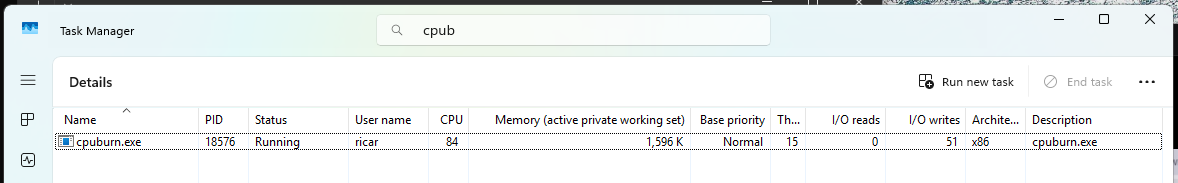
\includegraphics[width=\linewidth]{../imagenes/Administrador-tareas.png}
	  \caption{El proceso CPUBurn desde el administrador de tareas.}
	  \label{fig:cpuburn-administrador-tareas}
	\end{figure}

      \item Entre las ventajas de la afinidad de procesos se encuentran: un mejor rendimiento de la cache, ya que no hay que estar moviendo los datos de una cache a otra para que los puedan utilizar distintos procesadores; también permite evitar que procesos compitan por el mismo núcleo. Algunas desventajas, sin embargo, de la afinidad son: una posible reducción del rendimiento y que si el núcleo asignado está muy ocupado, el proceso que tienen afinidad a dicho núcleo no se va a ejecutar hasta que este se libere; ademas, le quitamos flexibilidad al sistema operativo ya que lo forzamos a asignar ciertos procesos a núcleos predeterminados.
	\begin{figure}[H]
	  \centering
	  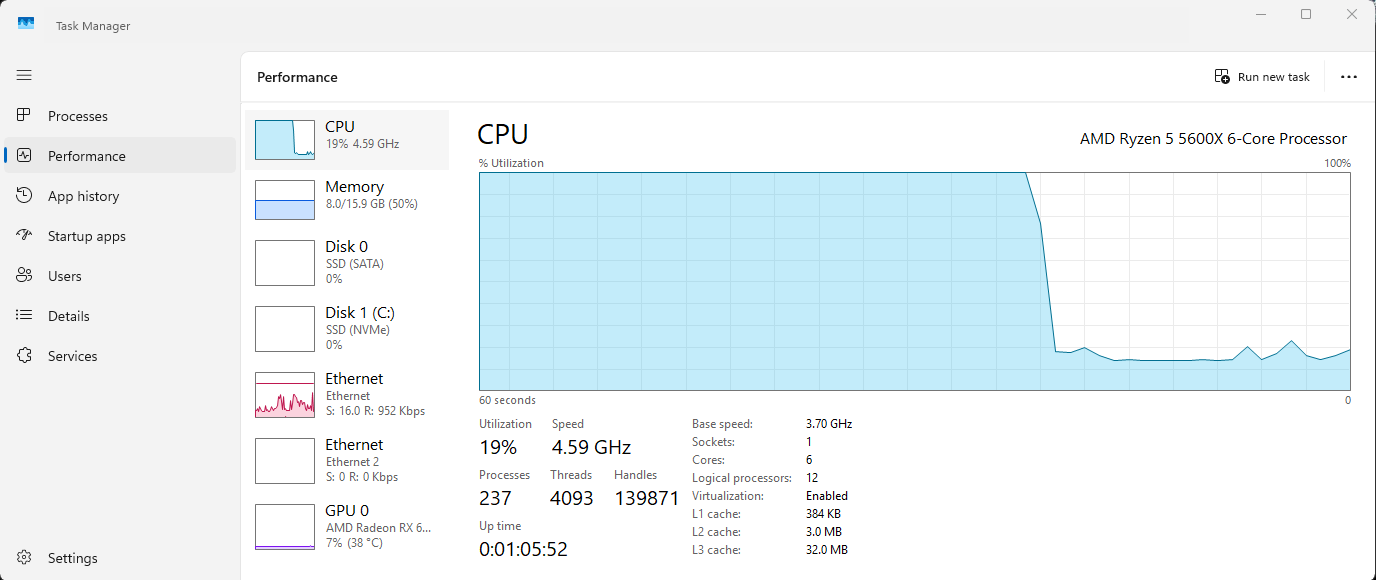
\includegraphics[width=\linewidth]{../imagenes/cpuburn-un-procesador.png}
	  \label{fig:cpuburn-afinidad}
	  \caption{El proceso CPUBurn con afinidad a un solo núcleo.}
	\end{figure}

      \item Para suspender a CPUBurn había pensado en hacer click derecho en el proceso desde el Administrador de Tareas y darle a la opción Suspender, pero no existía esa opción. Tampoco sé de la existencia de un comando en la consola de Windows para suspender un proceso, así que opté por suspenderlo desde la aplicaión Process Explorer.
	\begin{figure}[H]
	  \centering
	  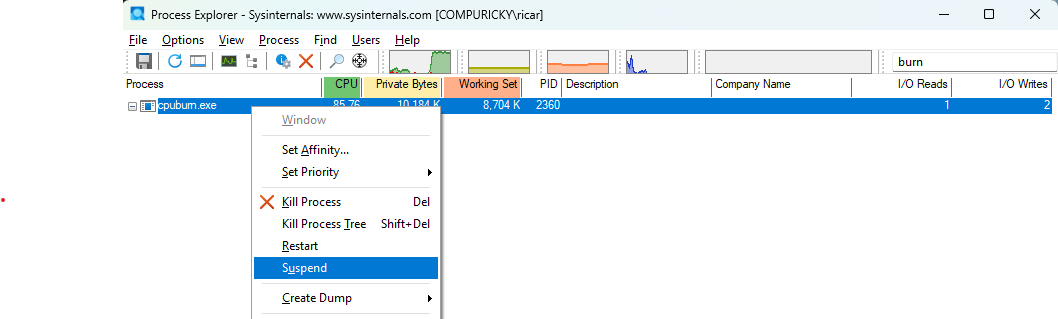
\includegraphics[width=\linewidth]{../imagenes/cpuburn-suspend.png}
	  \caption{Suspendiendo el proceso CPUBurn desde la aplicación Process Explorer.}
	  \label{fig:cpuburn-suspend}
	\end{figure}

      \item Para finalizar el proceso hago click derecho sobr el proceso CPUBurn desde el Administrador de Tareas y selecciono la opción ``Finalizar Tarea''.
	\begin{figure}[H]
	  \centering
	  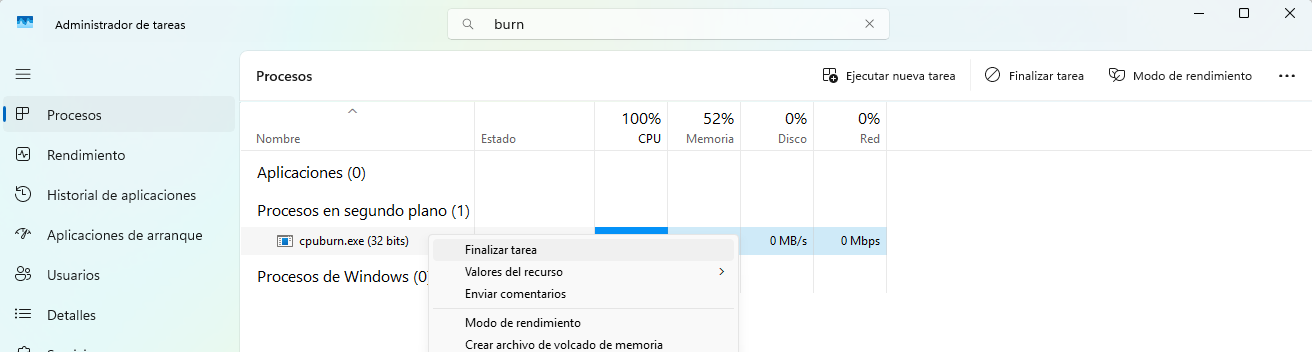
\includegraphics[width=\linewidth]{../imagenes/cpuburn-finalizar.png}
	  \caption{Finalizando el proceso CPUBurn desde el Administrador de Tareas.}
	  \label{cpuburn-finalizar}
	\end{figure}
    \end{enumerate}

    \item Sí se puede notar la diferencia entre programa y proceso. Un programa es un conjuntos de instrucciones escritas en algún lenguaje y almacenadas en un archivo. Este no está en ejecución. Por otro lado, un proceso es un programa en ejecución, y por ende abarca también todos los recursos asociados a la ejecución de ese programa. En las imagenes vemos que cuando no se realizan cambios en el archivo .txt, este se comporta como un programa, ya que no hay ningún CPU ejecutando instrucciones. Sin embargo, en el momento en que se empieza a escribir sobre ese archivo, se le asigna un CPU, aumenta la cantidad de memoria utilizada, la lectruras y escrituras de entrada y salida.
      \begin{figure}[H]
        \centering
        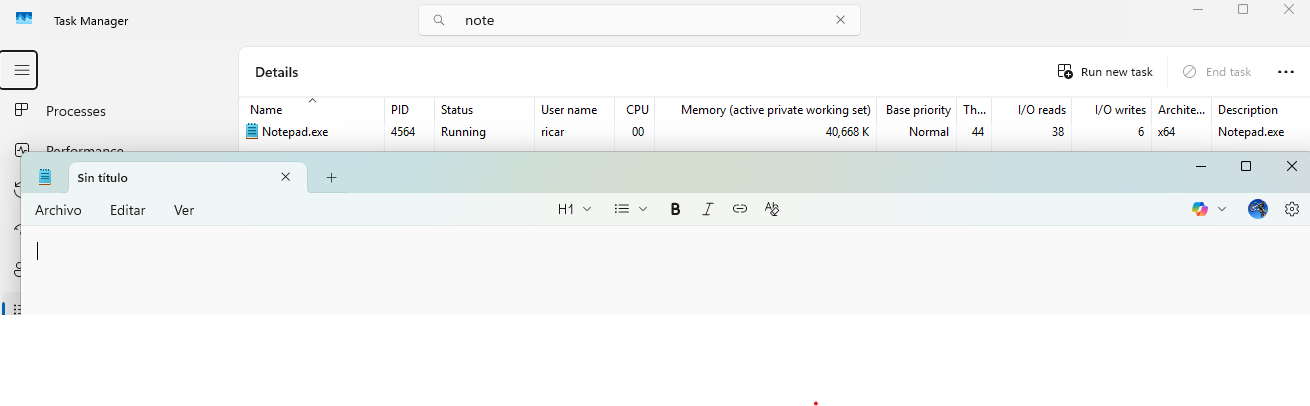
\includegraphics[width=\linewidth]{../imagenes/bloc-notas-sin-escribir.png}
        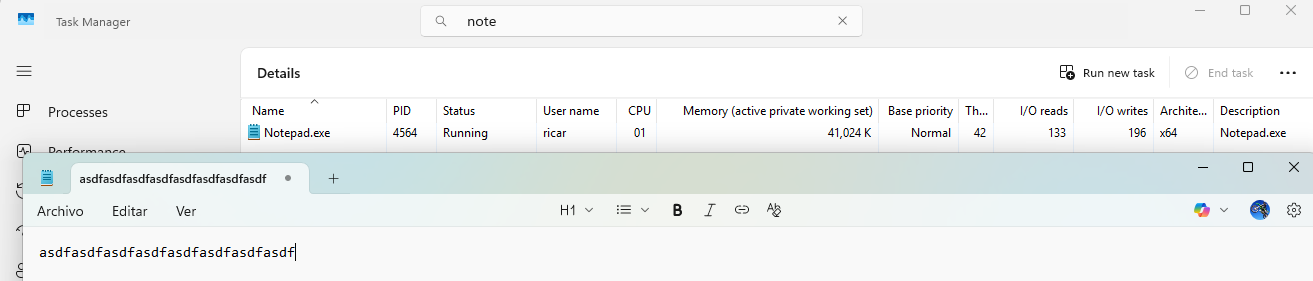
\includegraphics[width=\linewidth]{../imagenes/bloc-notas-escribiendo.png}
        \caption{Diferencia entre programa y proceso.}
        \label{programa-vs-proceso}
      \end{figure}

    \item Una vez abierto Process Explorer y Virtual Box: 
      \begin{enumerate}[]
	  \item [a,b.] Sí se puede ver la ejecución de la máquina virtual desde Process Explorer.
	    \begin{figure}[H]
	      \centering
	      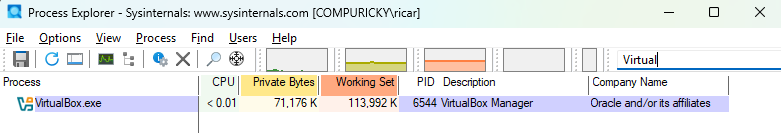
\includegraphics[width=\linewidth]{../imagenes/virtualbox-ejecutando.png}
	      \caption{Ejecución de Virtual Box vista desde Process Explorer.}
	      \label{vm-ejecutando}
	    \end{figure}

	  \item [c,d.] En las siguientes figuras se puede ver el uso del CPU durante la ejecución del comando \verb|find| en la máquina virtual.
	    \begin{figure}[H]
	      \centering
	      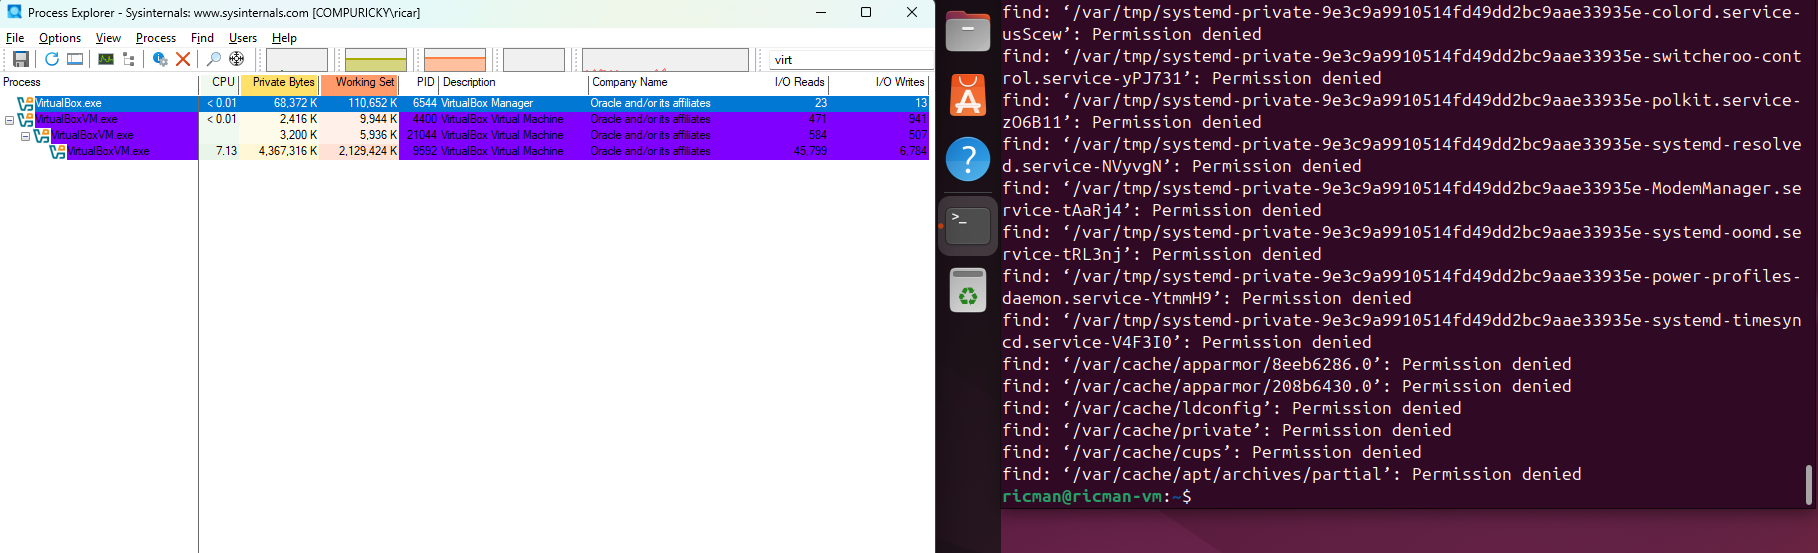
\includegraphics[width=\linewidth]{../imagenes/vm-find.png}
	      \caption{Uso del CPU y E/S durante la ejecución del comando \texttt{find} en la máquina virtual.}
	      \label{vm-find}
	    \end{figure}

	  \item [e.] Si intento suspender el proceso ``raiz'' de Virtual Box, me aparece un error que me dice que no tengo los permisos necesarios para realizar la acción. 

	    Sí puedo suspender los otros procesos hijos del proceso raíz, pero esto no tiene efecto en la máquina virtual y la puedo usar con normalidad.
	    \begin{figure}[H]
	      \centering
	      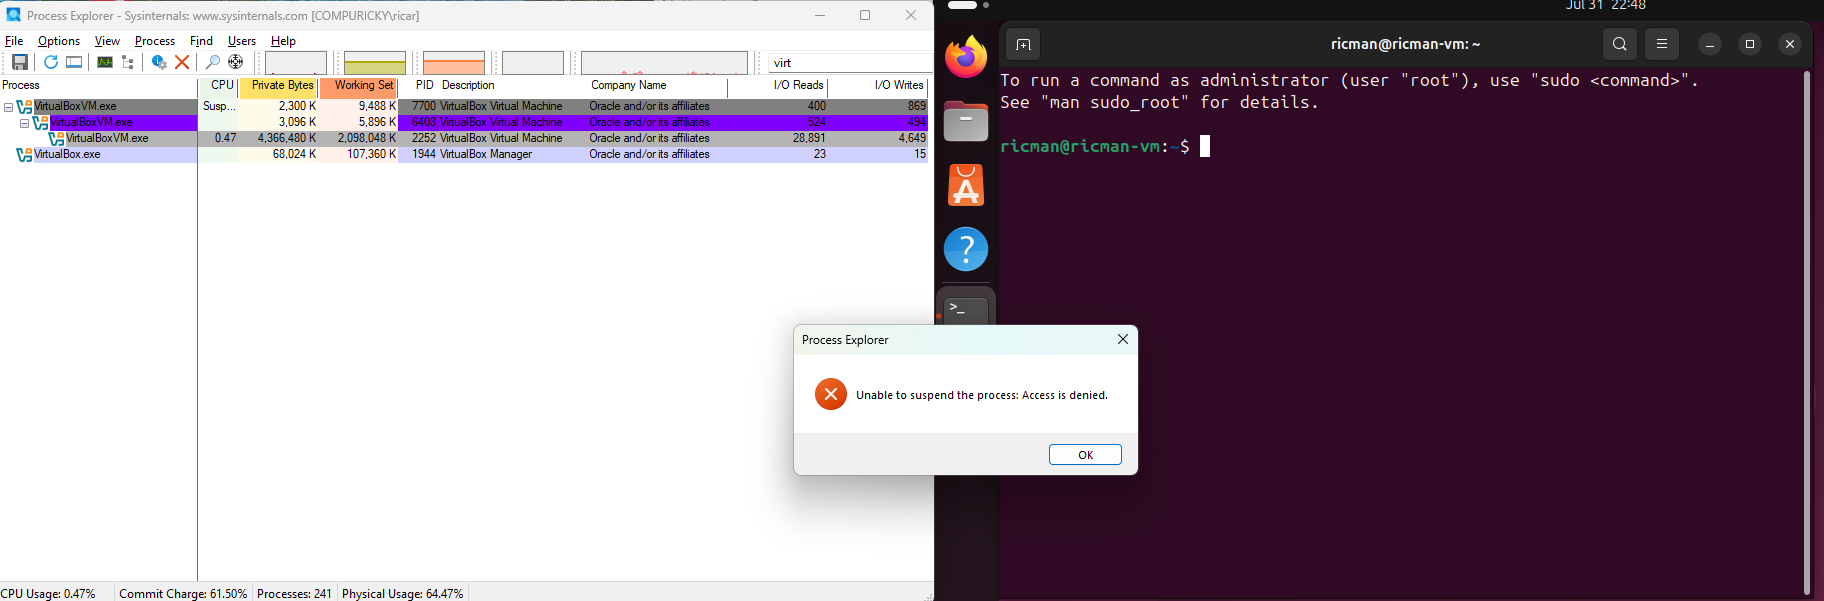
\includegraphics[width=\linewidth]{../imagenes/suspend-vm-denied.png}
	      \caption{Denegado el intento de suspensión del proceso raíz de la máquina virtual.}
	      \label{}
	    \end{figure}
	    \begin{figure}[H]
	      \centering
	      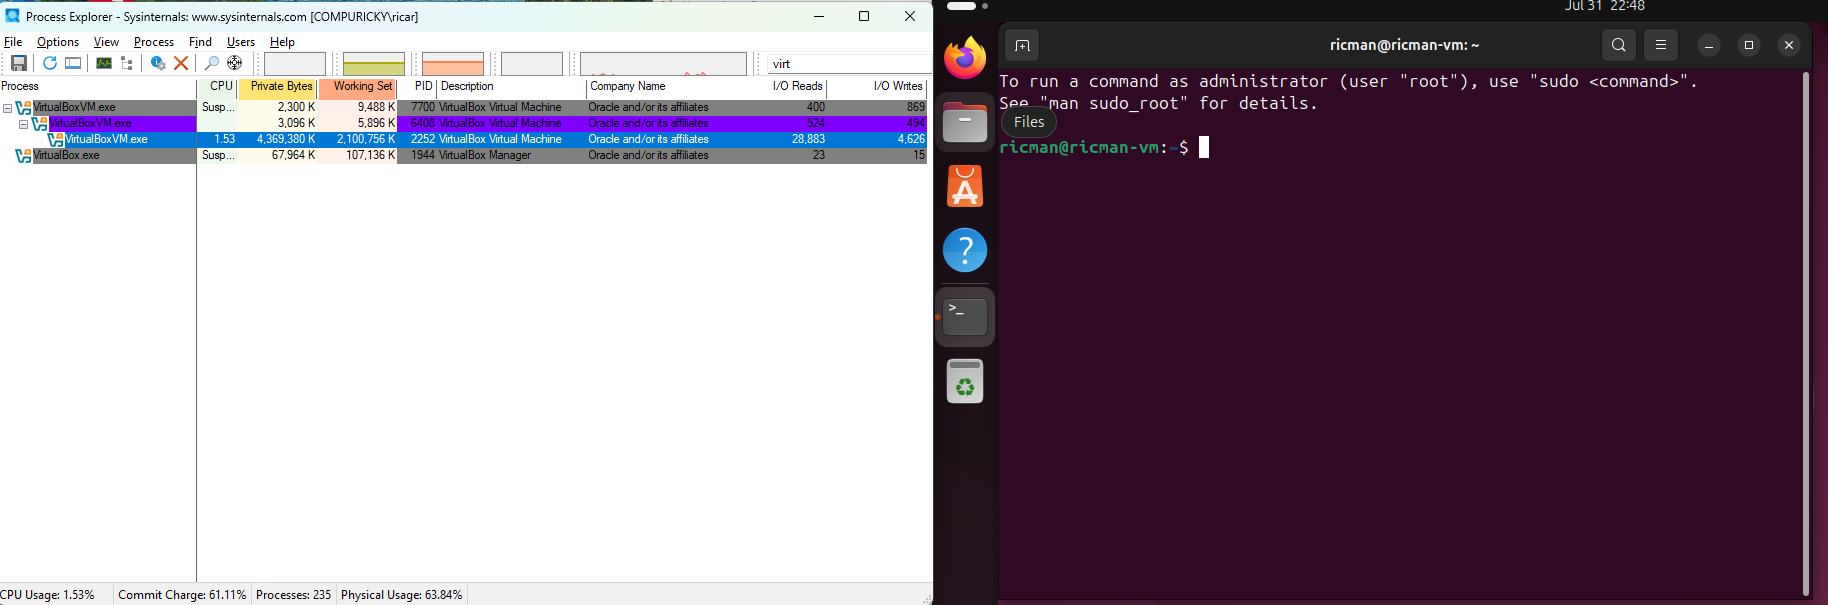
\includegraphics[width=\linewidth]{../imagenes/suspend-vm.png}
	      \caption{Sub-procesos de la máquina virtual suspendidos.}
	      \label{}
	    \end{figure}
      \end{enumerate}

      \item Debido a que el resultado de la ejecución de Handle para mostrar los archivos abiertos del navegador (Brave en mi caso) tenía una gran cantidad de líneas, considero mas conveniente presentar dicho resultado en un formato de texto, en vez de varias capturas de pantalla. 

	Al ejecutar el comando \verb| handle64.exe "C:\windows\system32" | se imprimió en la consola lo siguiente:
     \begin{lstlisting}[style=consola]
brave.exe          pid: 21444  type: File           628: C:\Windows\System32\en-US\kernel32.dll.mui
brave.exe          pid: 21444  type: File           6D4: C:\Windows\System32\drivers\etc
brave.exe          pid: 21444  type: File           BF0: C:\Windows\System32\en-US\user32.dll.mui
brave.exe          pid: 21444  type: File           BF4: C:\Windows\System32\en-US\propsys.dll.mui
brave.exe          pid: 21444  type: File          16E8: C:\Windows\System32\en-US\KernelBase.dll.mui
brave.exe          pid: 21444  type: File          17D0: C:\Windows\System32\en-US\Windows.FileExplorer.Common.dll.mui
brave.exe          pid: 13396  type: File           D68: C:\Windows\System32\en-US\KernelBase.dll.mui
brave.exe          pid: 21404  type: File           350: C:\Windows\System32\drivers\etc
brave.exe          pid: 8648   type: File           350: C:\Windows\System32\en-US\MMDevAPI.dll.mui
brave.exe          pid: 8612   type: File          1004: C:\Windows\System32\en-US\propsys.dll.mui
     \end{lstlisting} 

      \item Muestra todos los archivos que tiene abierto el kernel de windows. Entre ellos se pueden ver los archivos correspondientes al navegador brave, que es el que estaba siendo utilizado en ese momento.

      \item En este punto primero se abrió una terminal (la que está a la derecha en las imágenes) en la que se corrió el comando \verb|top|. Luego, en otra terminal se corrió el comando \verb|ps aux| para ver todos los procesos que se estaban ejecutando en ese momento. Además se utilizó un pipeline con grep top para filtrar solo los procesos que contengan el nombre \verb|top| y que sea mas facil encontrar el proceso buscado. 
	\begin{figure}[H]
	  \centering
	  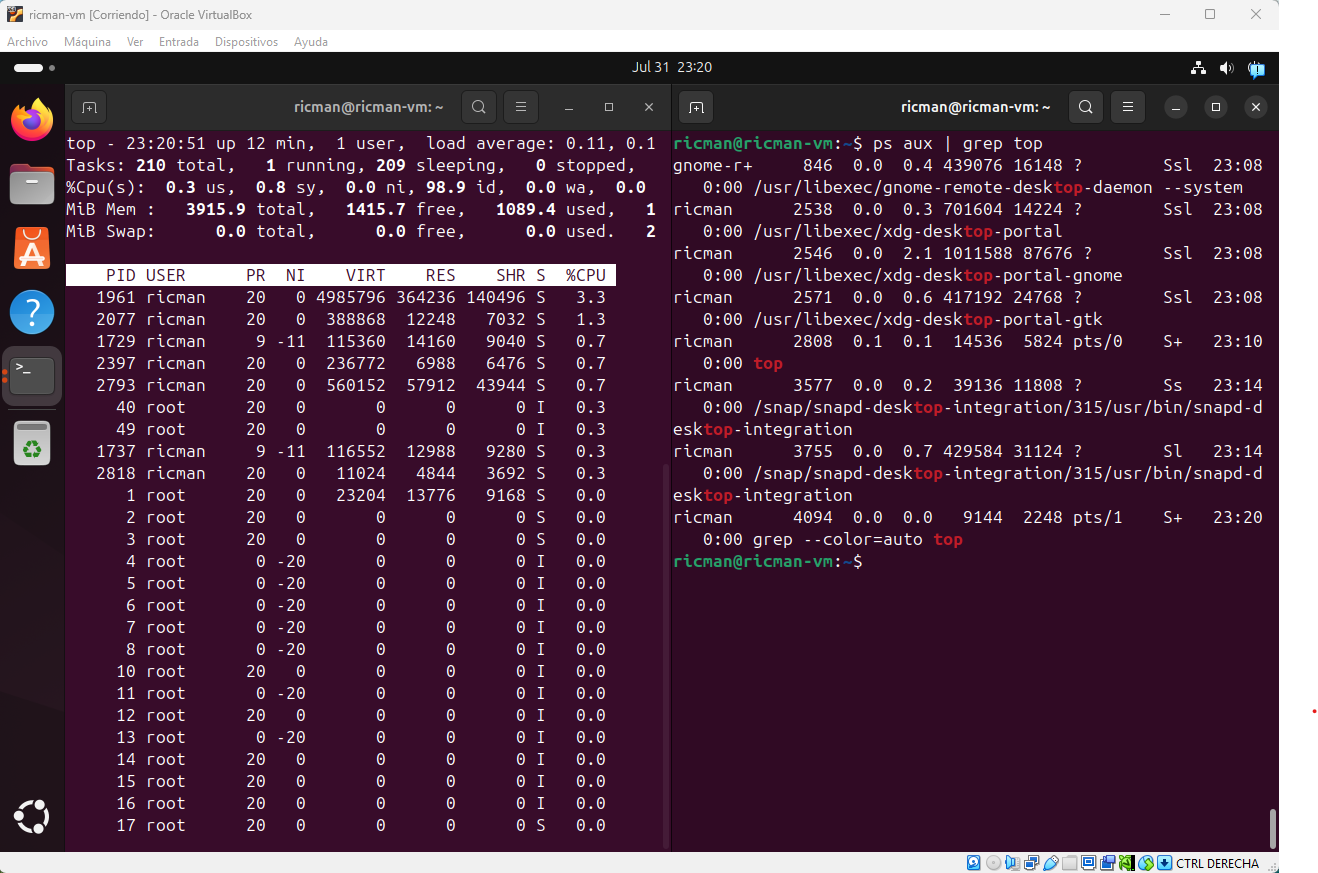
\includegraphics[width=\linewidth]{../imagenes/top-corriendo.png}
	  \caption{El proceso \texttt{top} corriendo en la terminal izquierda, y su PID en la derecha.}
	  \label{}
	\end{figure}

	Luego, una vez identificado el proceso con el PID (en este caso 2808), se ejecutó el proceso \verb|kill -SIGINT 2808| para enviarle el mensaje especificado.
	\begin{figure}[H]
	  \centering
	  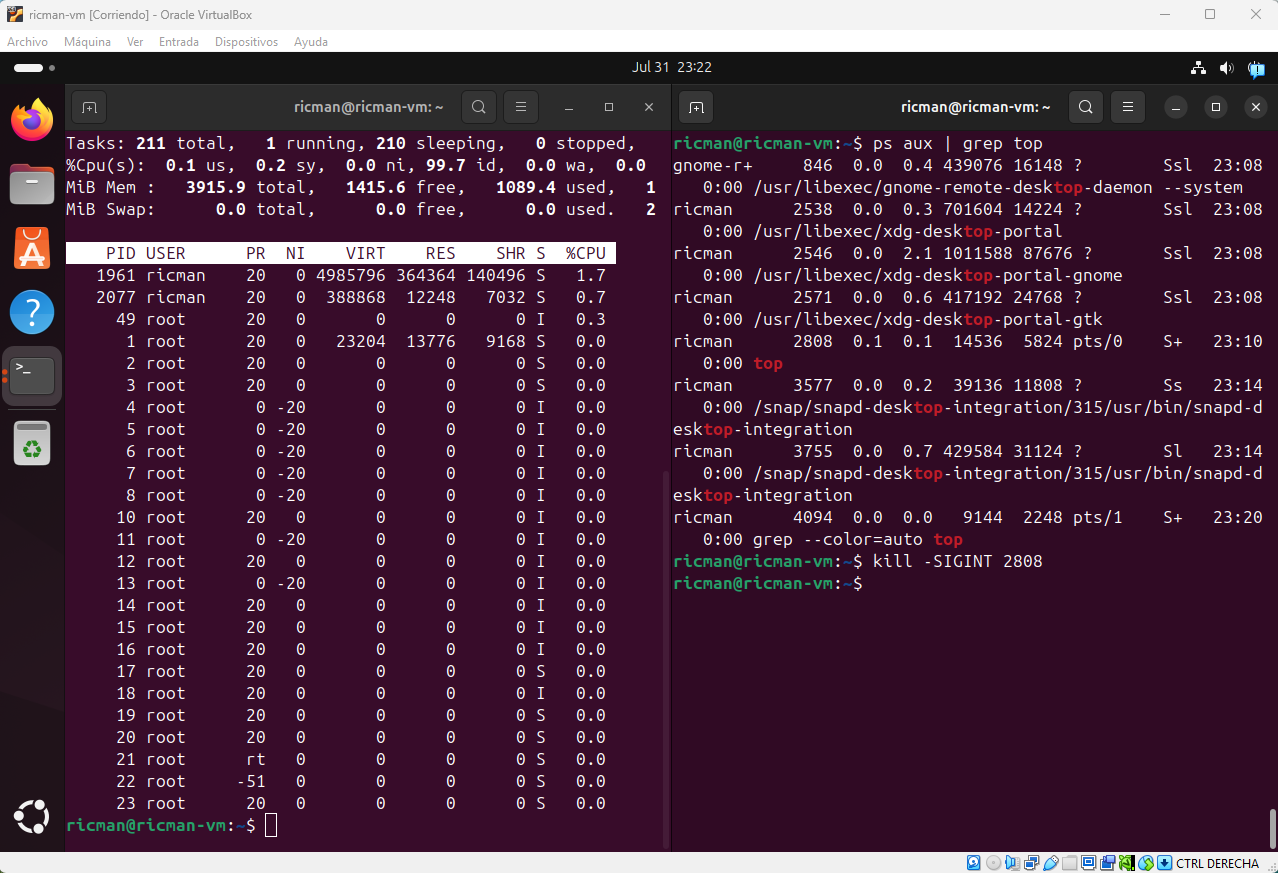
\includegraphics[width=\linewidth]{../imagenes/top-despues-de-parar.png}
	  \caption{El proceso \texttt{top} finalizado luego de enviarle la señal \texttt{SIGINT}.}
	  \label{}
	\end{figure}

    \item En la siguiente figura se puede ver cómo se volvió a ejecutar el comando \verb|top| en la terminal de la izquierda, mientras que en la terminal de la derecha se volvió a buscar el PID del proceso para programar su finalización a las 02:34 hs.
      \begin{figure}[H]
        \centering
        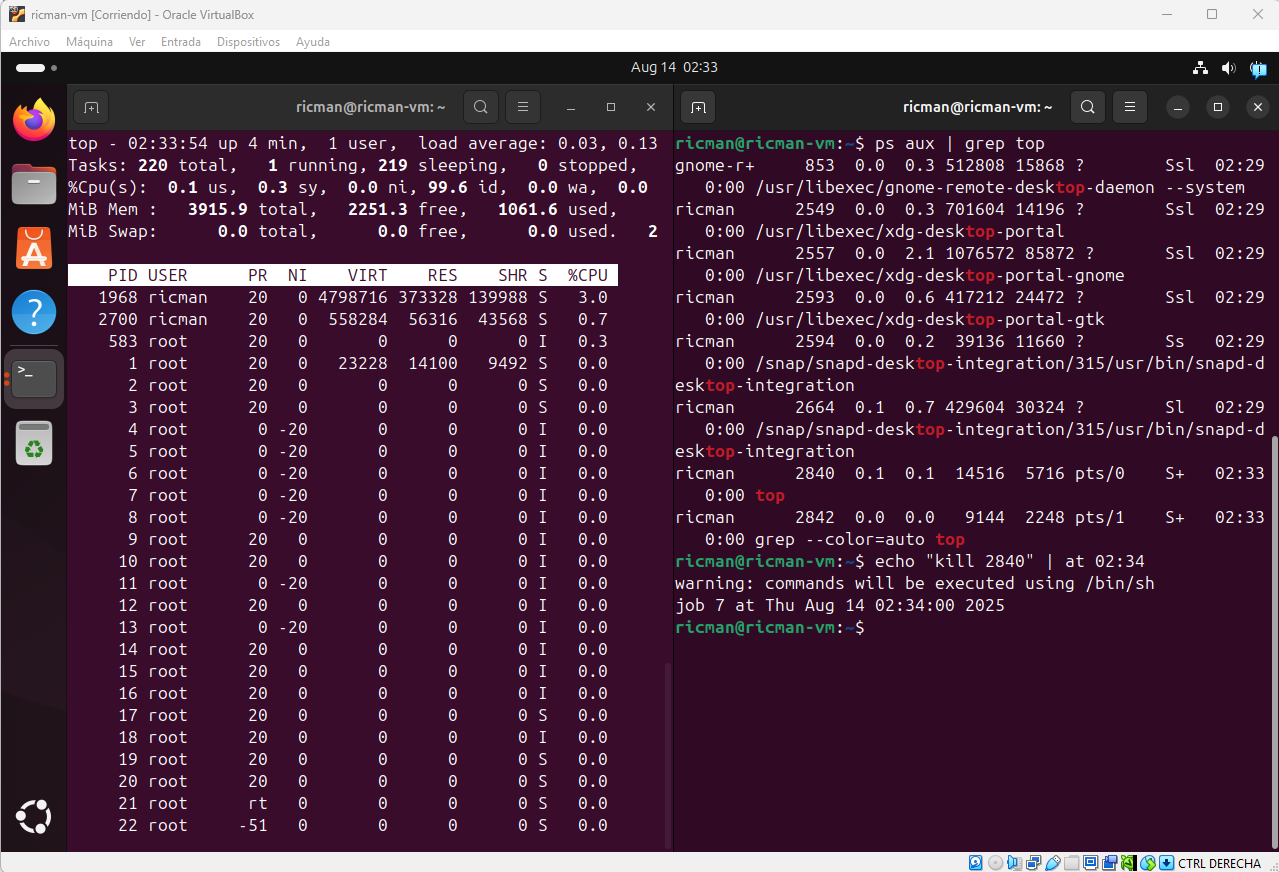
\includegraphics[width=\linewidth]{../imagenes/top-corriendo-at.png}
        \caption{El comando \texttt{top} ejecutándose a las 02:33 y programado para finalizar a las 02:34.}
        \label{top-corriendo-at}
      \end{figure}

      En la siguiente figura se puede ver cómo, efectivamente, a las 02:34 el proceso \verb|top| finaliza su ejecución.
      \begin{figure}[H]
        \centering
        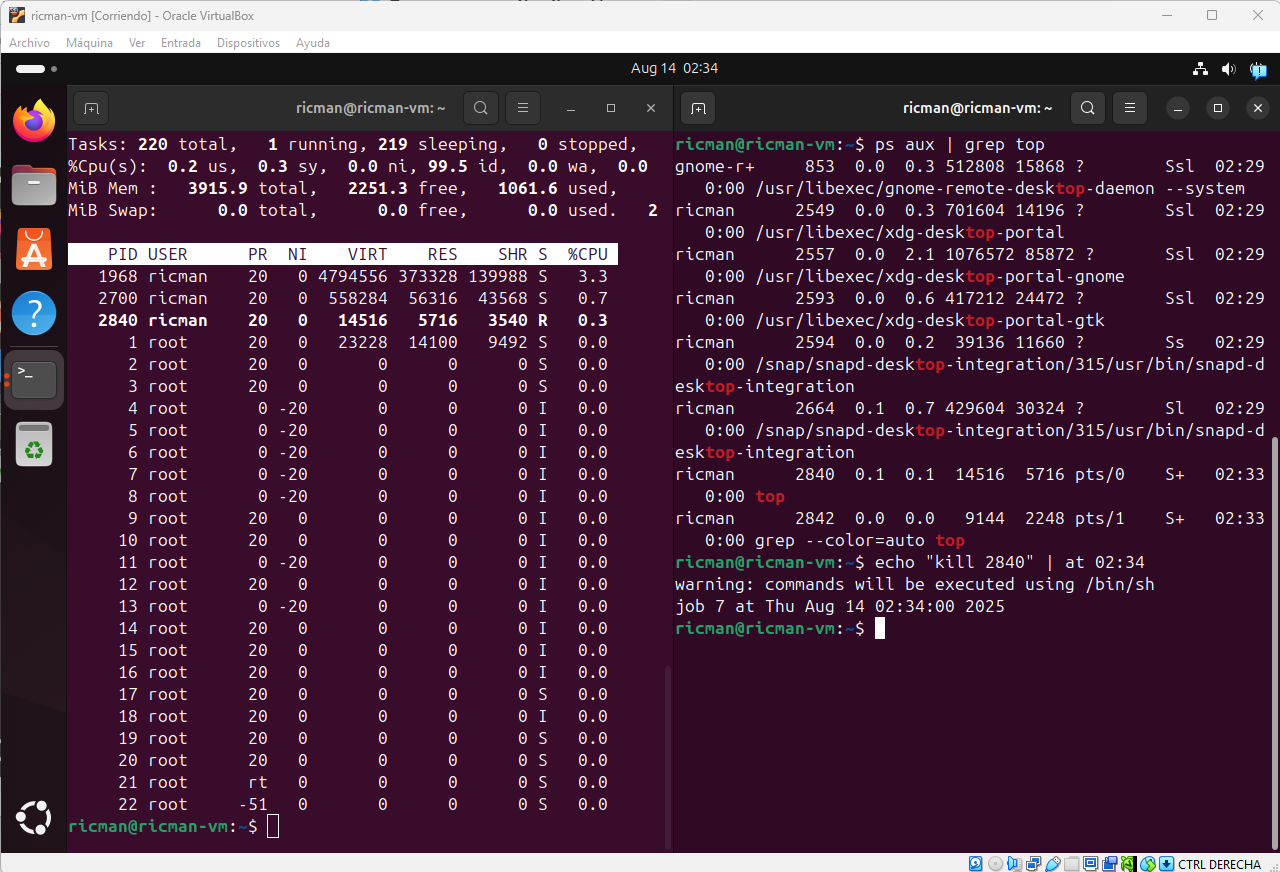
\includegraphics[width=\linewidth]{../imagenes/top-parado-at.png}
	\caption{El proceso \texttt{top} finalizado a las 02:34.}
        \label{top-parado-at}
      \end{figure}
  \end{enumerate}

  \section{Conclusión}
  El trabajo práctico sirvió para comprender las diferentes formas de gestionar los procesos en Windows y Linux, y también logró resaltar la importancia que tiene el poder comprender y utilizar las herramientas disponibles en cada sistema operativo para monitorear y controlar los procesos. En Windows la forma de gestionar los procesos es principalmente mediante una interfaz gráfica, mientras que en Linux el enfoque se basa principalmente en el uso de comandos desde la terminal.

  %\newpage
  %\addcontentsline{toc}{section}{Referencias}
  %\printbibliography

\end{document}
